\documentclass{article}
\usepackage[left=2cm, right=2cm, top=0cm]{geometry}
\usepackage{amsmath}
\usepackage{amssymb}
\usepackage{fancyvrb}
\usepackage{xcolor}

\usepackage{graphicx}
\usepackage{enumitem}
\usepackage{algorithm}
\usepackage[noend]{algpseudocode}
\usepackage{tikz}
\usepackage{pgfplots}
\usepackage{hyperref}
\usepackage{lipsum}
\setlength\parindent{0pt}
% \hypersetup{
%    colorlinks,
%    citecolor=green,
%    filecolor=black,
%    linkcolor=blue,
%    urlcolor=blue
%}

\begin{document}
\title{Final Project: Roomba Coverage}
\author{Jacob Puthipiroj}
%\date{}
\maketitle

\begin{abstract}
	Roombas are autonomous vacuum cleaners equipped with a set of sensors designed to navigate and clean a room. Roombas can generally detect the presence of obstacles, determine if a spot is dirty or clean, and walls or steep drops in order to prevent it from falling down the stairs. In this final project, we attempt to simulate various strategies for roomba implementation, with the key metric being the number of steps taken.
\end{abstract}

\section*{Introduction}
In the following series of implementations, we consider a simplified model of a room to be cleaned as a represented as nodes on a graph. Certain simplifying assumptions have been made, including. 


\begin{itemize}[noitemsep]
\item \textbf{Room Layout:} The room is rectangular, and all obstacles are considered rectilinear.
\item \textbf{Obstacles:} Obstacles are generated the graph via the removal of nodes 
\item \textbf{Stopping Criterion:} The job of the Roomba terminates only when every single tile is cleaned. 
\item \textbf{Online Learning:} The Roomba does not have a prior knowledge of the layout of the map, and as a result must explore the layout of the room via certain 
\item \textbf{Infinite Battery:} The Roomba does not stop until its task is completely finished.
\end{itemize}


The conceptualization of the room as a graph is a highly useful as it allows for the borrowing of tools from network analysis (such as the min-cut to identity chokepoints in a room,), as well as search algorithms from graph theory (such as breadth-first search) which we will implement in this paper. (Framing the problem as a graph traversal) % think of min cut and dijkstra % also, decomposition

\section*{Strategies}
We consider three main strategies in this paper: 

% go into detail on each of the strategies. 

\subsection*{Random Movement}
In the most naive implementation, we simply move the Roomba to a random neighboring tile in the graph. The algorithm is as follows:  



\begin{algorithm}[h]
\caption{Random Movement}
\begin{algorithmic}[h]
\State {set all nodes to not visited}
\State {G[source\_node][`visited'] = True}
\State {current\_node = source\_node}

\State path = list()
\While {nodes in G not all visited}
\State neighbors = get\_neighbors(current\_node) 
\State next\_node = choice(neighbors)
\State G[next\_node][`visited'] = True
\State path.append((current\_node, next\_node))
\State current\_node = next\_node
\EndWhile	
\State return path
\end{algorithmic}
\end{algorithm} 


\newgeometry{left=2cm, right=2cm}
\subsection*{Depth-First Search}
Even without performing much analysis, it is easy to imagine that the random algorithm is going to be terribly inefficient. This Roomba does know where it has been or where it has to go for certain, and will move aimlessly until it has hopefully cleaned the entire room, which, if the room is large, may take an incredibly long time. Furthermore, in rooms with many hidden corners, e.g. where obstacles have created a 'U'-shape, certain nodes will have few, or perhaps only one edge leading to it, meaning that the Roomba will have to be very lucky to access all the nooks and crannies. Clearly, there are some improvements to be made. \\

Framing Roomba coverage as a graph traversal problem has a clear benefit, namely the ability to borrow algorithms and tools from graph theory. One prominent tool is that of depth-first search, which incidentally was created for solving mazes, a closely related traversal problem. The algorithm for depth-first search, with backtracing, is as follows\footnote{\#networks: I explain why I conceptualize the room as a network/graph, use relevant tools from graph theory, namely depth-first search to propose strategies for roomba searching. Of course, this requires some manual tweaking, because depth first search in its usual form does not include backtracing. }:

\begin{algorithm}[h]
\caption{Depth-First Search}	
\begin{algorithmic}[h]
\State {set all nodes to not visited}
\State {G[source\_node][`visited'] = True}
\State {current\_node = source\_node}
\State visited\_cells = list()
\State path = list()
\While {nodes in G not all visited}
\State neighbors = get\_unvisited\_neighbors(current\_node) 
\If{there are neighbors} 
\State visited\_cells.append(current\_node)
\State next\_cell = choice(neighbors)
\State G[next\_node][`visited'] = True
\Else 
\State next\_cell = visited\_cells.pop()
\EndIf
\State path.append((current\_node, next\_node))
\State current\_node = next\_node
\EndWhile
\State return path
\end{algorithmic}
\end{algorithm}

In the actual implementation in the corresponding Jupyter Notebook, we provide also the ability to choose the unvisited neighbor to traverse to deterministically, rather than leave it up to choice. 



\newgeometry{left=2cm, right=2cm}
\subsection*{Circular}
The depth-first search algorithm is likely to do better than the random algorithm; at least it is deterministically going to traverse the whole graph. What is likely to slow the DFS algorithm down, is its necessary but slow backtracing step. In the literature of coverage path planning, two ideas have been proposed: wall following, and spiralling. We combine both algorithms into a `circular' algorithm, which will traverse the graph by spiralling counter-clockwise around the source node, and follow the wall once it reaches it.\footnote{\#creativeheuristics: I researched and found multiple `heuristics', e.g. wall-following and spiralling, which I manage to integrate into the `circular' algorithm, along with explanations for how it works, and accompanying illustrations in the implementation section. I also critique this heuristic for its over-reliance on backtracing here and in the `Future Work' section, along with improvements.}
 
\begin{algorithm}[h]
\caption{Circular}	
\begin{algorithmic}[h]
\State {set all nodes to not visited}
\State {G[source\_node][`visited'] = True}
\State {current\_node = source\_node}
\State visited\_cells = list()
\State path = list()
\State direction = (np.array[[-1,0], [0,-1], [1,0], [0,1] ])
\State prev\_dir = 0
\While {nodes in G not all visited}
\State neighbors = get\_unvisited\_neighbors(current\_node) 
\If{there are neighbors} 
\State visited\_cells.append(current\_node)
\State next\_list = np.roll(direction, shift = -prev\_dir, axis = 0)
\State next\_list[[0,1,2,3]] = next\_list[[1,0,3,2]]
\ForAll {$i, j \in$ enumerate(next\_list)}
\If{$i$ + current\_node $\in $ neighbors}
\State prev\_dir = arg direction == $i$
\State next\_cell = $i$ + current\_node
\EndIf
\EndFor
\State next\_cell = choice(neighbors)
\State G[next\_node][`visited'] = True
\Else 
\State next\_cell = visited\_cells.pop()
\EndIf
\State path.append((current\_node, next\_node))
\State current\_node = next\_node
\EndWhile
\State return path
\end{algorithmic}
\end{algorithm}




% \textbf{Depth-First Search}: 
% \item \textbf{Circular}: This  \footnote{\#creativeheurstics:}
% \end{enumerate}
The result of this algorithm is that when the Roomba is initialized (sourced) in the middle of an empty room, the first node the Roomba will travel in is the one directly south, then east, then north, then west. Once the Roomba hits a wall, it will then attempt to follow it anticlockwise, but if the preferred cell has already been visited, it will then hug the wall the other way.  






% What do you want your simulation to be able to do and what information do you want to be able to measure from it?
% Describe the rules of your simulation and how they capture the situation you are modeling.
% Identify any modeling assumptions and explain under what circumstances these assumptions may and may not be valid.
% Describe the parameters of your simulation and how they affect the behavior of the simulation.
% Describe the output/measurements of your simulation and how they relate to the situation you are modeling. What are the quantities of interest?
\newgeometry{left=2cm, right=2cm}
\section*{Implementation}
\begin{figure}[h]
\centering
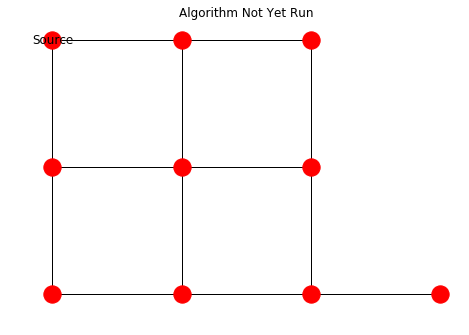
\includegraphics[width=8cm]{Base.png}
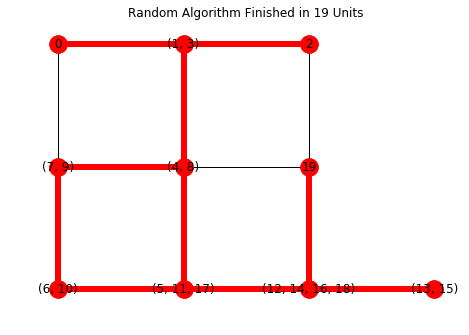
\includegraphics[width=8cm]{Random.png}
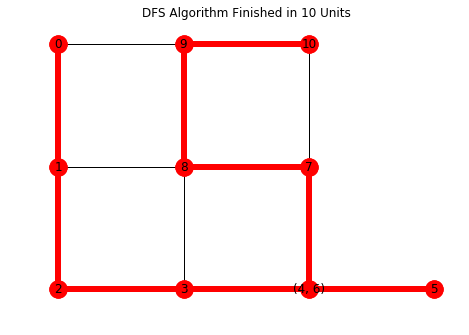
\includegraphics[width=8cm]{DFS.png}
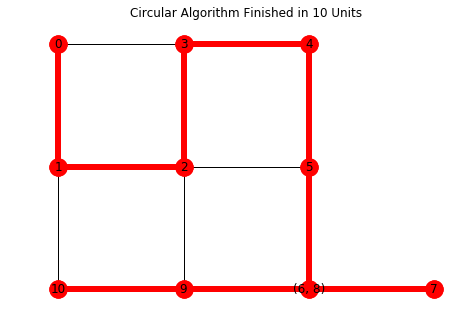
\includegraphics[width=8cm]{Circular.png}
\caption{In this simulation, the $4 \times 3$ room is initialized with 2 obstacles placed along with the wall, with the Roomba starting in the far corner. The random strategy takes the longest time, making several unnecessary back-and-forth steps, while the DFS and Circular algorithm tie.}

\end{figure}


% Implement your model in Python. (If you want to use a different programming language, please discuss with your course instructor first.) Make sure your code is correct, well-�structured, and readable - use interpretable variable names, comments, and doc strings.

\section*{Interpretation}
These four illustrations are highly typical of the behavior of strategies in used by the random, DFS and circular algorithms. Notice that an optimal path taking only 9 edge lengths is possible, but undiscovered. The Random algorithm is highly inefficient, visiting nodes already previously visited, up to 4 times in the case of the tile at $(2,0)$. However, the random algorithm also creates a loop in the graph, a behavior not seen in the path of the DFS or circular algorithm, as the latter are algorithms mainly used for searching trees, and are not meant to take advantage of the formulation of the room as an strongly connected undirected graph.

% What is the distribution over the outputs of your simulation? Visualize, describe andanalyze your results.

% If possible, describe what you think the probability distribution followed by yourmeasurements is.

% Write a paragraph or two to advise someone on the best action to take based onyour results - for example, in the parcel routing topic below, what should thedelivery company do to optimize the utilization of their delivery vans? Write thisparagraph in a style that is appropriate to your audience - for example, a managerof the delivery company.

\newgeometry{left=2cm, right=2cm}


\section*{Analysis and Comparison}
An obvious question is to ask how the total path length taken to traverse the entire graph scale as a function of the room size. 	In the simplest case, we consider when the room is square, and the room is completely empty. Therefore, the only factor is the starting node. As seen in the following graphs, the path length of the average DFS traversal is both longer and shows greater variance, i.e. uncertainty, than the Circular algorithm. The circular algorithm is so much more consistent, in fact, that even the 97.5\% upper bound for a $10  \times 10 $ room is 110. In a room of 100 tiles, this indicates near perfect traversal despite starting in a rather inefficient location. The lower end of the confidence interval for both are quite closely, indicating that the best runtimes for both algorithms are similar, but the worst of the DFS algorithm far exceeds the worst runtime of the Circular algorithm.\footnote{\#confidenceintervals: Interpreted confidence intervals for the path lengths of the two deterministic algorithms, noting that we are trying to use confidence intervals to generalize and abstract away the one random parameter, that is the source node.} 

\begin{figure}[h]

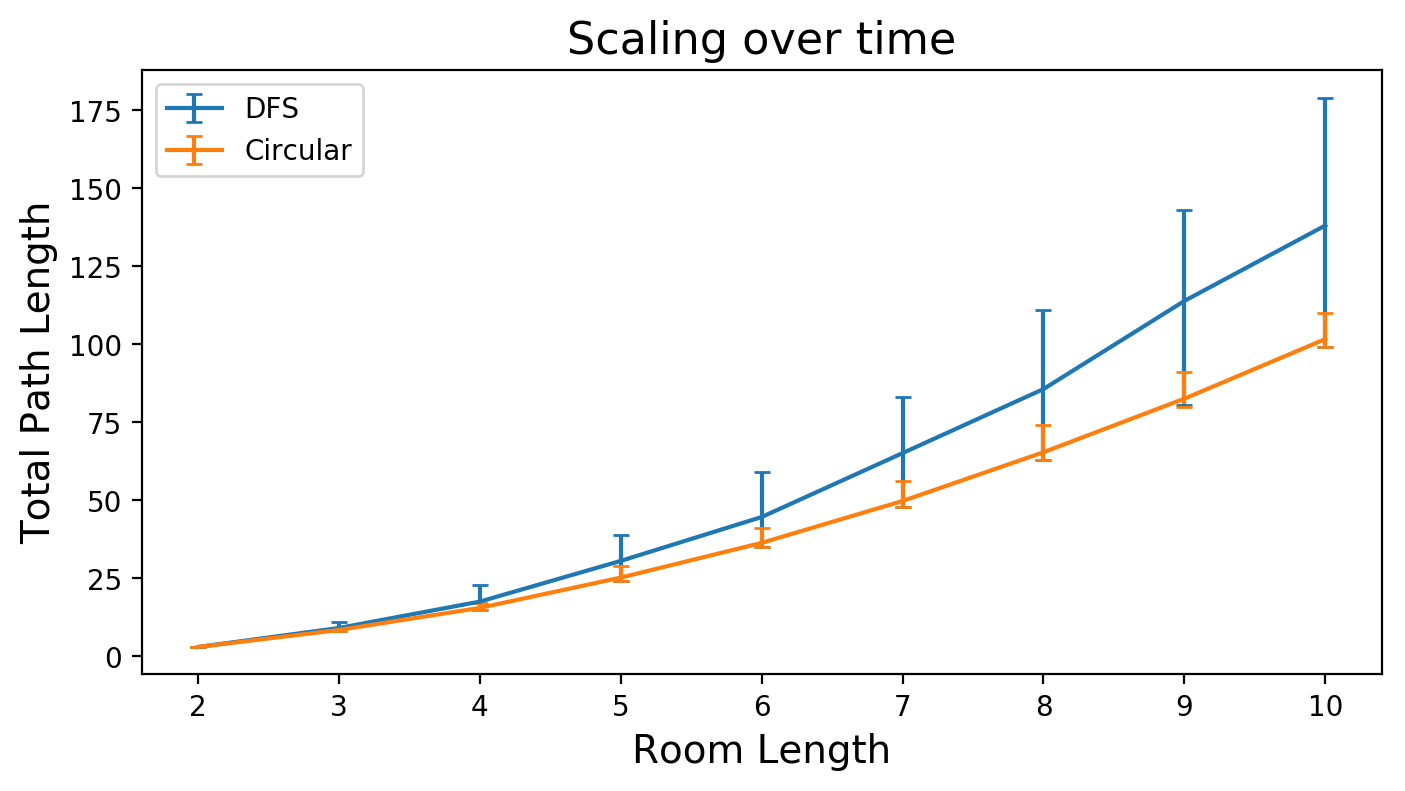
\includegraphics[width=8cm, ]{scalingcomparison.png}
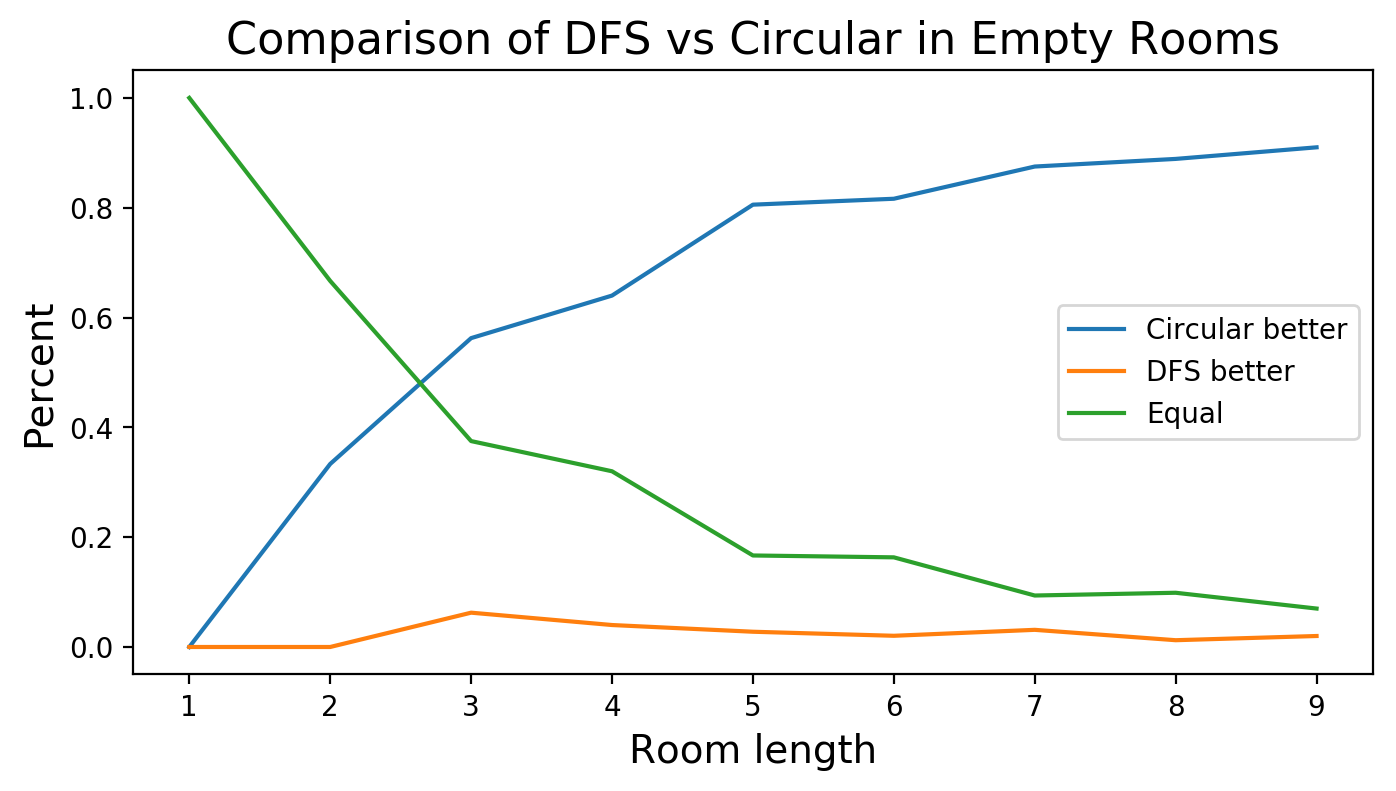
\includegraphics[width=8cm]{Circularvsdfsempty.png}
\centering
\end{figure}

\subsection*{What happens when there are obstacles?}
The introduction of obstacles into the simulation makes comparison of the two algorithms much more interesting. Whereas in the case of the empty square room where there were $n$ unique situations, where $n$ is the length of the room, including $k$ obstacles would give $\binom{n^2}{k}\times (n^2-k)$. This number is an overestimation, since some configurations of obstacles cut the graph into multiple disjoint nodes which are not strongly connected. 

\begin{figure}[H]
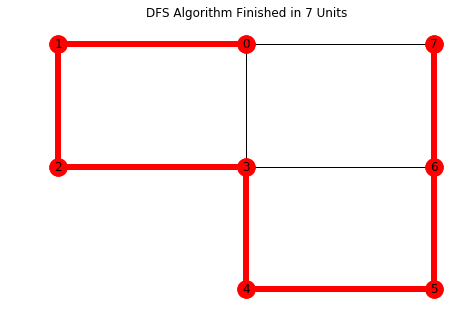
\includegraphics[width=8cm]{dfs_faster.png}
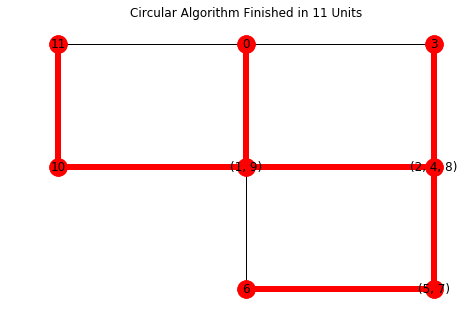
\includegraphics[width=8cm]{circular_slower.png}
\end{figure}

In this particular configuration of obstacles and having (1,2) as a starting node, we see the DFS algorithm actually outperforming the circular algorithm. From the figure, it would seem that when the rooms are not empty, the differences between the the DFS and circular algorithm do not seem as cut and dry as they originally did. Indeed, a 3d plot of the performances of both the DFS circular algorithm show little obvious differences.


\subsection*{When is DFS faster than Circular?}
Even in the base case of a square room without obstacles, the DFS algorithm does sometimes provide a more efficient path than the circular algorithm. Because of the deterministic nature of both algorithms, the DFS is faster than the circular algorithm if and only if the roomba starts on very particular nodes. In a $2 \times 2$ or a $3 \times 3$ room without obstacles, this never happens. On a $4 \times 4$, $5 \times 5$, $6 \times 6$ and $7 \times 7$ grid, this happens only once out of all possible starting locations, and the DFS is only marginally faster, gaining an edge of 2, 2, 4 and 2 steps respectively. In a $8 \times 8$ grid, the DFS algorithm is faster in 2 out of 64 possible starting positions. Compared to the vast majority of cases in which the circular algorithm is faster, and by a much larger margin, this seems trivial. The following table enumerates all of unique configurations of simulations in a square empty room. 


\begin{table}[h]
\centering
\begin{tabular}{|l|l|l|l|l|l|l|l|l|l|}

\hline
\textbf{Grid Type}                & \textbf{2x2} & \textbf{3x3} & \textbf{4x4} & \textbf{5x5} & \textbf{6x6} & \textbf{7x7} & \textbf{8x8} & \textbf{9x9} & \textbf{10x10} \\ \hline
\textbf{DFS Faster}      & 0            & 0            & 1            & 1            & 1            & 1            & 2            & 1            & 2              \\ \cline{1-1}
\textbf{Circular Faster} & 0            & 3            & 9            & 16           & 29           & 40           & 56           & 72           & 91             \\ \cline{1-1}
\textbf{Equal}           & 4            & 6            & 6            & 8            & 6            & 8            & 6            & 8            & 7              \\ \hline
\textbf{Total}           & 4            & 9            & 16           & 25           & 36           & 49           & 64           & 81           & 100            \\ \hline
\end{tabular}
\end{table}



\subsection*{Distributions of DFS and Circular}
A close examination of the `scaling over time' plot shows an interesting result. As a result of the circular algorithm's extreme efficiency in empty rooms, there is a distinct difference in the skew of the distributions of the total path length. The mean performance of the DFS algorithm seems always to be roughly in the middle of the two confidence intervals each time. However, the distributions of the circular algorithm is continually right-skewed: the mass of the distribution is concentrated near the left of the distribution, where the optimal performance is. When obstacles are introduced to the simulation, this drastically changes.   

\begin{figure}[H]

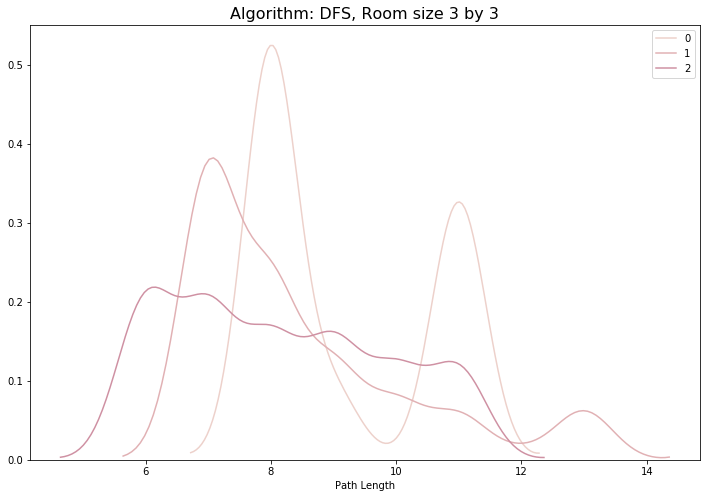
\includegraphics[width=8cm]{dfs_3.png}
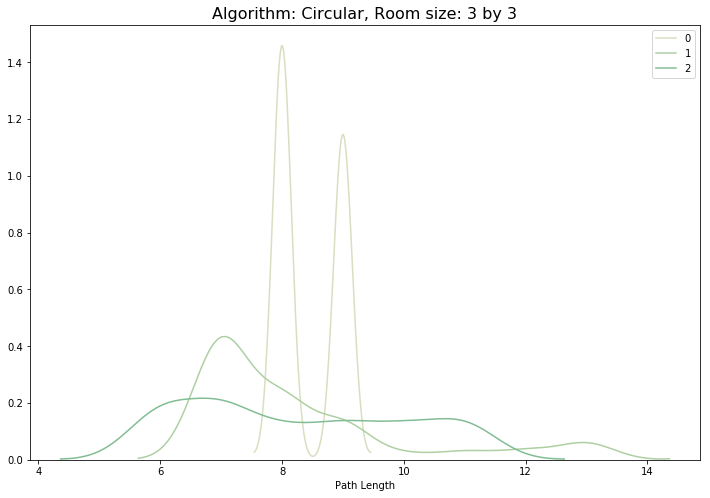
\includegraphics[width=8cm]{circular_3.png}
\centering
\end{figure}
\begin{figure}
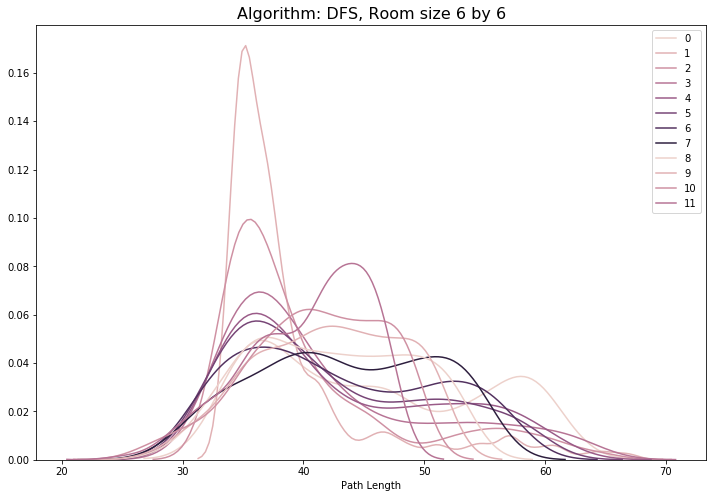
\includegraphics[width=8cm]{dfs_6.png}
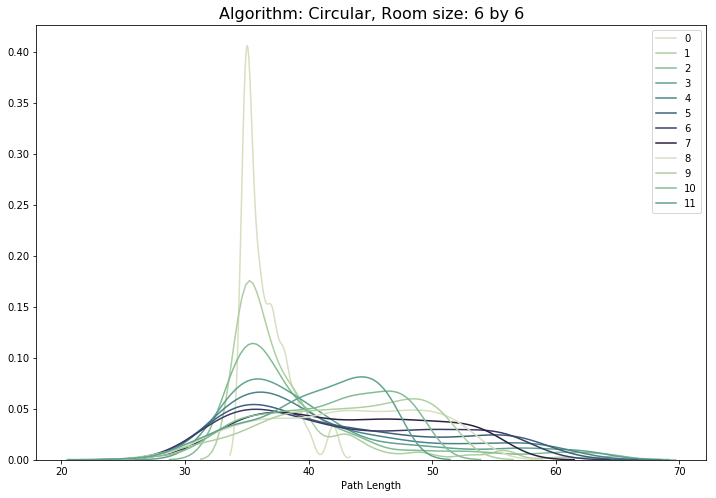
\includegraphics[width=8cm]{circular_6.png}
% 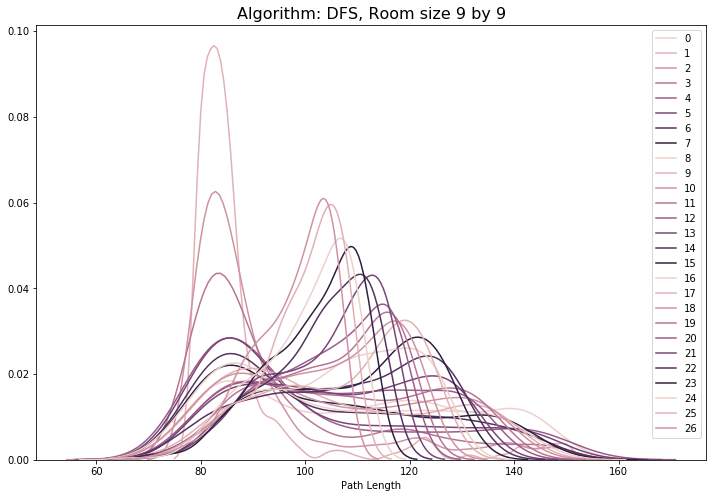
\includegraphics[width=8cm]{dfs_9.png}
% 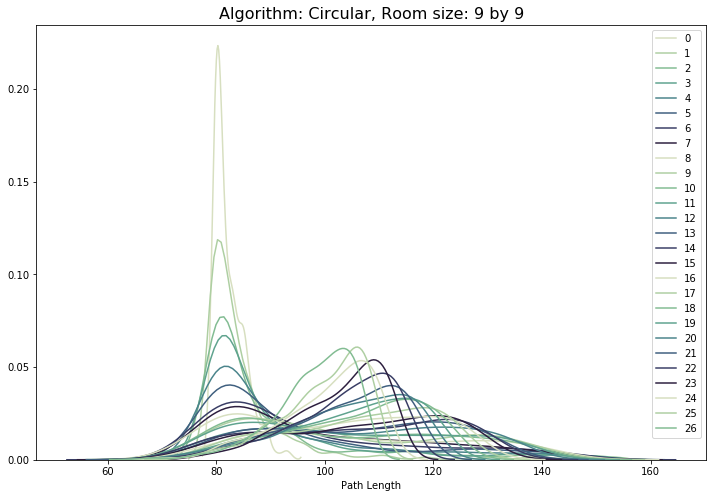
\includegraphics[width=8cm]{circular_9.png}
\centering
\end{figure}
The four plots above are density plots; showing a smoothed, continuous version of a histogram estimated from data. Specifically, we see how the addition of obstacles to a 3 by 3 square room affects the distribution of path lengths, with the lines indicating successively increasing numbers of obstacles. As obstacles are added (as the lines grow darker in shade), performance of both algorithms go from being left-skewed to gradually more right-skewed. One clear major difference between the two is that the Circular algorithm performs far better on emptier rooms, and is most optimal when there are no obstacles at all. In that case, the performance of the circular is far superior to the DFS algorithm. This advantage rapidly decays, however, with performance in 1-obstacle rooms being already almost identical in the $3  \times 3$ room, and with roughly equal performance at 5 obstacles in the $6 \times 6$ room. \\


Also interesting is the bimodal nature of the underlying distributions when there are fewer obstacles in the room. This is most prominent in the case of the $3 \times 3$ room, where the performance of both algorithms in an empty room show peaks at 8 and 11 path edges. This likely corresponds to frequent initialization patterns in the room layout - when the room is $3 \times 3$, there are 9 tiles, and if the Roomba can traverse them perfectly, then the performance is 8 edge lengths. However, it is not actually possible to have a performance of 10 edge lengths, because deviations from the optimal path necessarily require one forward and one backtracing step from already visited nodes, and then one more in the direction of the unvisited node. As the number of obstacles increases, this multimodal behavior vanishes, as the distributions flatten out and resemble a uniform distribution, before reemerging as a left-skewed unimodal distribution. At no point do the path length seem to strongly follow a univaraite Gaussian distribution; instead the flat, roughly uniform shape indicates the equilibrium number of obstacles per room for both algorithms. In fact, the logic stemming from the bimodal shape distribution in the $3 \times 3$ indicates that the final shape of the distribution is a composition of multiple smaller ones, akin to a Gaussian mixture model of multiple degenerate Gaussians (there is no variance for each individual Gaussian, as the output is a discrete integer).\footnote{\#distributions: Identifying the change in the distributions for total length as the number of obstacles in the room increases, by referencing a shift from a bimodal/multimodal distribution to a flatter uniform, and then to a left-skewed distribution, and interpreting this as a gaussian mixture model of degenerate Gaussians, with a resulting shift in the means of the individual Gaussian.}\\

To see the aforementioned changes in the changes in greater detail, we turn to two common descriptive statistics for non-normal data, namely the skew and kurtosis. In order to consider the changes in skew and kurtosis as greater numbers of obstacles are added to a room, we rely on a 3-dimensional approach which incorporates both the room length, number of obstacles and our parameter of interest.\\

\begin{figure}[h]
\centering
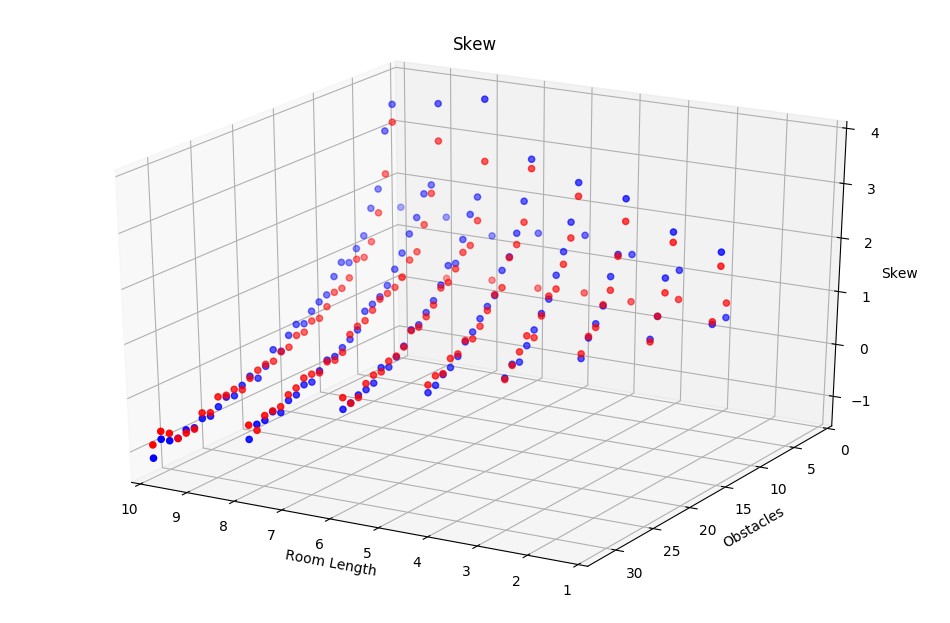
\includegraphics[width=8cm]{Skew.png}
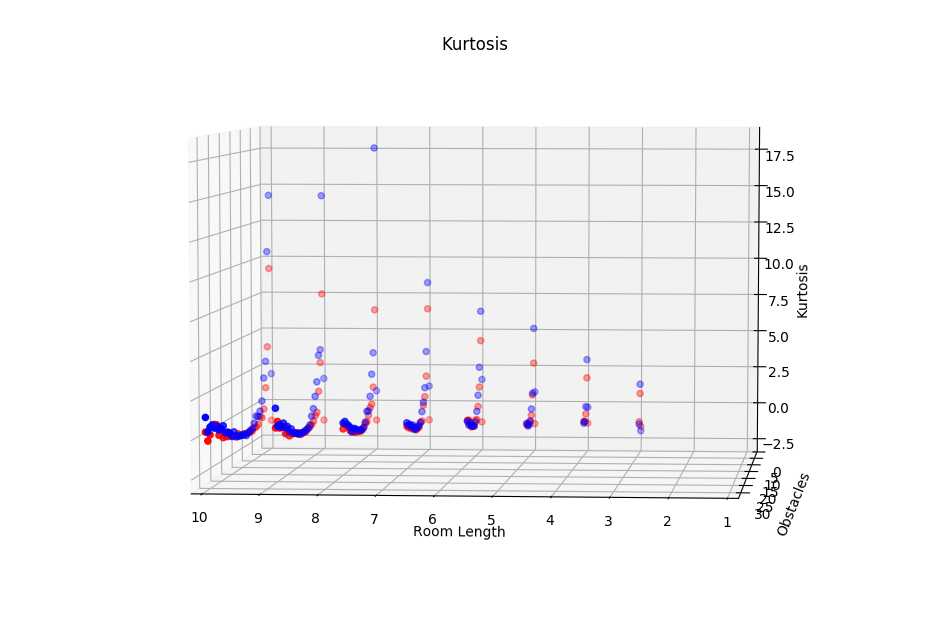
\includegraphics[width=8cm]{Kurtosis.png}
\end{figure}


In the above figures, the red and blue  dots correspond to the DFS and circular algorithm respectively. From the plot on the left, it is immediately clear that our observation of the changing skews in distribution as the number of obstacles increase is confirmed. A positive skew indicates that the mass of the distribution is concentrated on the. left, in context corresponding to lower path length and being skewed towards lower runtimes. A consequence of having heavily skewed distributions, whether to the left or to the right, is that many common inferential tools, such as confidence intervals may become invalid because of their implicit assumption of normality. \\

The plot on the right portrays the kurtosis of the distributions. Kurtosis refers to the `tailedness' of the distributions, where positive kurtosis indicates having fatter tails, like the exponential distribution. Negative kurtosis indicates having thinner tails, like the uniform distribution. Indeed, this is what we observed in the density plots: in an empty room, the distribution starts off with positive skew and kurtosis, like an exponential distribution, then has around zero skew with negative kurtosis, like a uniform distribution, then finally settles into a negative-skewed, positive kurtosis distribution (one real-life distribution of this shape is the life expectancy distribution in developed nations). Having explored appropriate descriptive statistics, we turn to confidence intervals, keeping in mind its questionable validity.\footnote{\#descriptivestats: I choose skewness and kurtosis, two appropriate choices for descriptive statistics, justifying my choice that the distribution is non-normal thus requires nonparametric metrics. I then provide an explanation for why the distribution's skew and kurtosis changes over time. I also generate `histograms' in the form of density plots.}


\begin{figure}[h]
\centering
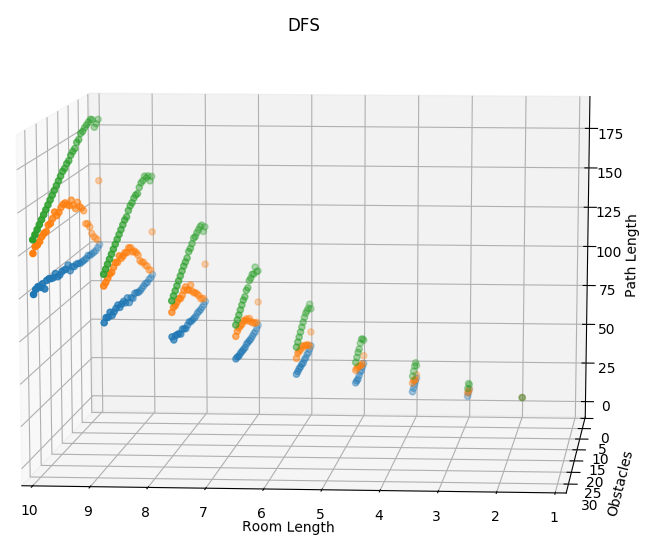
\includegraphics[width=8cm]{newdfsobstacles.png}
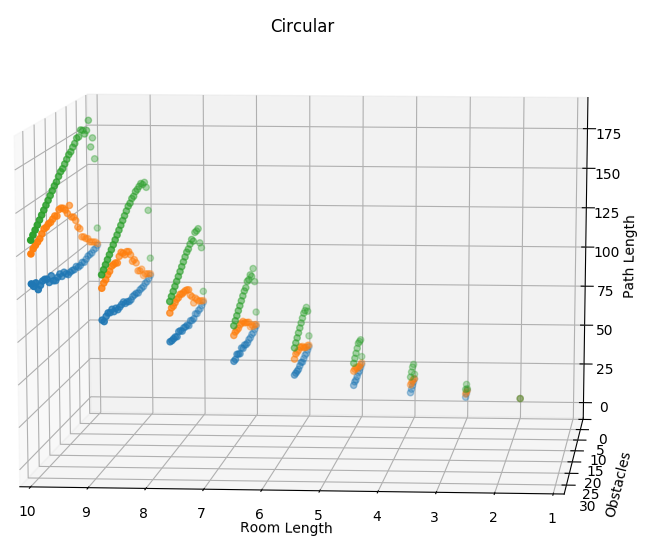
\includegraphics[width=8cm]{newcircularobstacles.png}s
\end{figure}


In these figures, the green, orange and blue dots correspond to the mean, the lower and  the upper bound for a 95\% confidence interval for the path lengths of a Roomba for a square room given a certain number of obstacles. Our preliminary 'base' case of empty rooms is empirically confirmed by the small number of green dots in the back which curve up towards a rapid peak in the Circular algorithm 3d plot - these patterns do not appear in the DFS algorithm. Another interesting pattern are the bell-shaped peaks of the mean for both algorithms - it would appear that the introduction of obstacles is indeed frustrating for the Roomba, but only up until a certain point, at which the obstacles have filled the graph up so much that the Roomba need only `follow the walls' to reach every tile!\\ 

What is most surprising are how similar the two peaks of the mean distribution seem, especially for larger room sizes. Two subtle differences are firstly that the trajectory of the mean distribution leading up to the peak in larger rooms seems to be concave for the DFS, but convex for the Circular algorithm, suggesting that the quality of the latter rapidly degrades as more obstacles are added to the room. A second observation is that the peaks of the lower bound seem more pronounced in the circular algorithm than the DFS algorithm, suggesting that DFS performs slightly better in heavily congested rooms. Indeed, this seems intuitive, since the DFS algorithm was first developed for solving mazes. \\



Of course, to confirm these hypotheses and avoid simple p-hacking, we must perform significance tests. 
\subsection*{Significance Tests}
Similar to the above plots, which extends the idea of a confidence interval beyond the 2d plot and into three dimensions, we perform a large number of significance tests, one for each configuration with the same room length and obstacles, and plot the results of the significance test a 3d plane. As for the test, we cannot use a t-test, as a t-test assumes normality of the underlying distribution. A quick normality test in scipy showed that the samples were extremely unlikely to have come from a normal distribution, and as such we use a nonparametric test, the Mann-Whitney U Test.\footnote{\#significance: I apply the Mann-Whitney U test and show the significance levels for said test on two 3d plots, explaining my choice of using a nonparametric test with reference to the failed normality test on the dataset. This is also clearly a complex use case, and I have to address the multiple-comparisons problem.}\\







\begin{figure}[h]
\centering
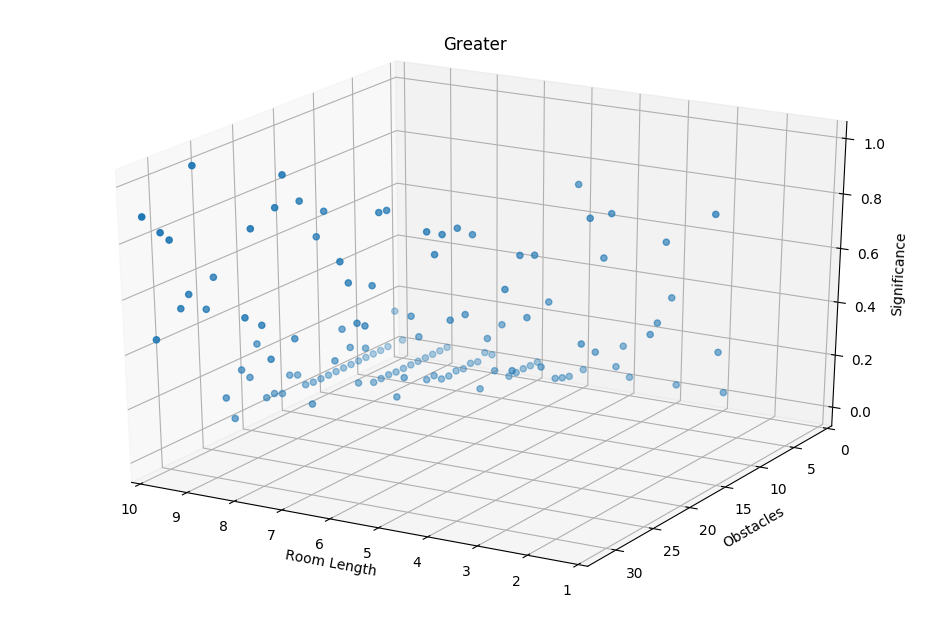
\includegraphics[width=8cm]{greater.png}
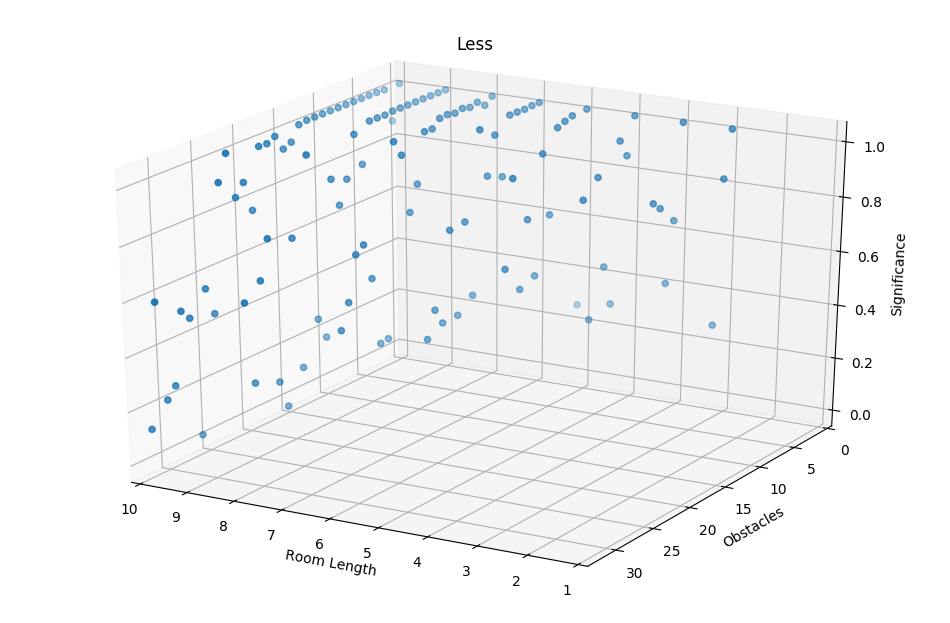
\includegraphics[width=8cm]{less.png}
\end{figure}
Here, the plots display the significance level of the Mann-Whitney U test for the DFS algorithm taking a greater (or less, respectively) path length than the Circular algorithm. It is immediately clear from the right plot that our second hypothesis, of the DFS performing better in rooms with many obstacles is likely false, as we fail to reject the null hypothesis anywhere on the plot. On the other hand, our suspicion that the circular algorithm performs better on average than the DFS algorithm in larger, open rooms is now empirically confirmed - although exactly how much larger ---the question of practical, rather than statistical significance--- is another matter entirely. \\

Briefly worth mentioning is that in many other contexts, performing such a multitude of comparisons is likely going to lead to erroneous inferences stemming from an inflated Type-I error, in a process akin to p-hacking. In this particular implementation, however, we are not extrapolating results from one specific tests out of many, but empirically confirming a mathematical truth -- of statistically significant differences between the DFS and the Circular algorithm in larger, open rooms, which we have also established before.



% Analyze the remaining uncertainty in your results. This is a Monte Carlo simulation, so themore simulation runs you do, the more certain you can be about your results.

% Provide 95% confidence intervals on the expected values of the quantities you aremeasuring.


% Comment on how many more simulations or simulation steps would you need toreduce the widths of your confidence intervals



% #confidenceintervals: Apply and interpret confidence intervals. (C) FA
% #simulation: Apply and interpret simulation modeling. (C) FA
% #professionalism: Follow established guidelines to present yourself and your work products professionally. (H) MC
% #audience: Tailor oral and written work by considering the situation and perspective of the people receiving it. (H) MC
% #cs166-mcmodeling: Model or interpret probabilistic state transitions for Monte Carlo simulations of non-deterministic scenarios.
% #cs166-mcanalysis: Given a stochastic model, apply concepts and techniques from Monte Carlo theory to analyze the characteristics of the model.
% #cs166-pythonimplementation: Given a description of the state space and update rules of a model, implement a simulation of the model in Python.
% #cs166-interpretresults: Summarize, interpret and communicate conclusions or results from analyzing models and simulations.

\section*{Future Work}
Although we have considered the two deterministic algorithms, the DFS and the Circular algorithm in detail, it would seem that there is much improvement to be made. Specifically, the backtracing element of the depth first search, used in both the circular and vanilla algorithm remains a source of inefficiency. In the future, we can imagine a more optimal path going from a dead end to any unvisited nodes, which can emulate the feature of shortcuts that the random algorithm takes. This is simple to implement, and relies on the Roomba having its own personal mental map of the room, consisting of visited nodes and their immediate neighbors. Once a Roomba has reached a dead end, it need only implement Dijkstra's shortest path algorithm to find and get to the the nearest unvisited node, from where it can continue with the circular algorithm.\footnote{\#networks: Another use of graph theory to help generate solutions, although not actually implemented}.\\
	 
A second deficit of the model which makes it unfit for production is the assumption of infinite battery life. Real Roombas has a limited battery life, although some have the feature to recharge themselves by guiding itself to a charging dock once it is low on battery. This is also a relatively easy addition that was not made based on time constraints, but would involve the Roomba keeping track of how far away it is from the charging node in terms of battery life. When it is low on battery, it can simply use Dijkstra's algorithm to get to the charging dock in a recursive fashion similar to the backtracing of the DFS and Circular algorithm. \\

Finally, the analysis could have been improved by considering the effect of having rooms of various proportions. The majority of this paper was focused on the interaction between obstacle sizes, algorithms, and starting nodes, but barely considered how a rectangular room, like a corridor, would affect the performance of the algorithm. Of course, a rectangular room is functionally no different from a square room with obstacles along the walls in multiple layers, but this was not explicitly considered.

\section*{Appendix}
The code used to generate the simulation and plots are available in the accompanying Jupyter Notebook, as well as online \href{https://github.com/thetruejacob/CS166/blob/master/Network%20Simulation%20Assignment/Network%20Simulation.ipynb}{here}.


% Current algorithms for decision trees, such as CART rely on sequential heuristics
% https://github.com/anarayanan86/MITx-6.00.2x
% https://github.com/lytemar/MIT-6.00.2x/blob/master/ProblemSet2/ps2.py
% https://github.com/EDalSanto/MIT-6.00.2x/blob/master/ProblemSet2:%20iRobot/ps2_visualize.py
% https://github.com/Boykai/Roomba-Vaccuming-Robot-Sim/blob/master/ps2.py
% https://courses.edx.org/courses/course-v1:MITx+6.00.2x+1T2019/courseware/d39541ec36564a88af34d319a2f16bd7/dec06bd802704d7cbc341dddd6c3306f/1?activate_block_id=block-v1%3AMITx%2B6.00.2x%2B1T2019%2Btype%40vertical%2Bblock%403f40a63fe6f145c9a0a5d6999ace816a


\end{document}